\documentclass[12pt,letterpaper]{article}

%%%%%%%%%%%%%%%%%%%%%%%%%%%%%%%%%%%%%%%%%%%%%%%%%%%%%%%%%%%%%%%%%%%%%%%%%
\pagestyle{plain}                                                      %%
%%%%%%%%%% EXACT 1in MARGINS %%%%%%%                                   %%
\setlength{\textwidth}{6.5in}     %%                                   %%
\setlength{\oddsidemargin}{0in}   %% (It is recommended that you       %%
\setlength{\evensidemargin}{0in}  %%  not change these parameters,     %%
\setlength{\textheight}{8.5in}    %%  at the risk of having your       %%
\setlength{\topmargin}{0in}       %%  proposal dismissed on the basis  %%
\setlength{\headheight}{0in}      %%  of incorrect formatting!!!)      %%
\setlength{\headsep}{0in}         %%                                   %%
\setlength{\footskip}{.5in}       %%                                   %%
%%%%%%%%%%%%%%%%%%%%%%%%%%%%%%%%%%%%                                   %%
\newcommand{\required}[1]{\section*{\hfil #1\hfil}}                    %%
\renewcommand{\refname}{\centerline{References Cited}}                 %%
\bibliographystyle{plain}                                              %%
%%%%%%%%%%%%%%%%%%%%%%%%%%%%%%%%%%%%%%%%%%%%%%%%%%%%%%%%%%%%%%%%%%%%%%%%%

%PUT YOUR MACROS HERE

\usepackage{graphicx}
\usepackage{subfigure}
\usepackage{amsmath}
\usepackage{amssymb}
\usepackage{times}
\usepackage{enumitem}
\usepackage{mathrsfs}
\usepackage[sort, compress]{natbib}
\usepackage{float}
\usepackage[ruled,vlined]{algorithm2e}
\usepackage{fixltx2e,dblfloatfix}
\usepackage{url}


\DeclareMathOperator*{\argmin}{argmin}
\DeclareMathOperator*{\argmax}{argmax}
\DeclareMathOperator*{\N}{\mathcal{N}}
\newcommand{\mbf}[1]{\mathbf{#1}} %note: I think using \mb killed the UF thesis template, changed to \mbf
\def\m{\textrm{m}}
\def\x{\mathbf{x}}
\def\t{\mathbf{t}}
\def\K{\mathbf{K}}
\def\y{\mathbf{y}}
\def\e{\mathbf{e}}
\def\p{\mathbf{p}}
\def\s{\mathbf{s}}
\def\b{\mathbf{b}}
\def\w{\mathbf{w}}
\def\n{\mathbf{n}}
\def\a{\mathbf{a}}
\def\u{\mathbf{u}}
\def\z{\mathbf{z}}
\def\B{\mathbf{B}}
\def\C{\mathbf{C}}
\def\E{\mathbf{E}}
\let\sec\S
\def\S{\mathbf{S}}
\def\I{\mathbf{I}}
\def\P{\mathbf{P}}
\def\X{\mathbf{X}}
\def\A{\mathbf{A}}
\def\C{\mathbf{C}}
\def\M{\mathbf{M}}
\def\U{\mathbf{U}}
\def\Y{\mathbf{Y}}
\def\Z{\mathbf{Z}}
\def\balpha{\boldsymbol\alpha}
\def\bmu{{\boldsymbol\mu}}
\def\btheta{{\boldsymbol\theta}}
\def\bSigma{\mathbf{\Sigma}}
\def\hbmu{\hat{\bmu}}
\def\hbSigma{\hat{\bSigma}}
\def\bTheta{\boldsymbol\Theta}
\def\bLambda{\boldsymbol\Lambda}
\def\del{\partial}
\newcommand{\bb}[1]{\textbf{#1}}

\usepackage[uppercase]{titlesec}
\titleformat{\section}{\bfseries \scshape \large }{\thesection}{1em}{}
\titleformat{\subsection}{\bfseries \scshape}{\thesubsection}{1em}{}
\titleformat{\subsubsection}{\bfseries \scshape}{\thesubsubsection}{1em}{}
\titleformat{\paragraph}{\bfseries}{}{1em}{}
\titlespacing*{\section}{0pt}{5pt}{0pt}
\titlespacing*{\subsection}{0pt}{5pt}{0pt}
\titlespacing*{\subsubsection}{0pt}{5pt}{0pt}
\titlespacing*{\paragraph}{0pt}{5pt}{0pt}



\title{Kernels \& Support Vector Machines Cont. }

\begin{document}
\maketitle

\section{Introduction to Support Vector Machines}
\begin{itemize}
\item SVMs are Maximum Margin Classifiers 
\item Two class classification problems: $y(\x) = \w^T\phi(\x) + b$

\item We cannot directly compute $\phi(\x)$ for all mappings, we want to use a kernel trick.  So, we have to write up a dual representation of the problem in terms of $K$ matrices
\item We will start with the case where the $\phi(x)$ are linearly separable in the kernel space
\item Note: the SVM finds a linear decision boundary in the feature space.  But since we can do non-linear transformations to get to the feature space, the descision boundary can be non-linear in the feature space. 
\item We want to find $\w$ and $b$ so that $y(\x) = \w^T\phi(\x) + b$ is $y(\x_n) > 0$ for $t_n = 1$ and $y(\x_n) < 0$ for $t_n = -1$.  Or, in other words, we want:
\begin{equation}
t_ny(\x_n) > 0 \forall n
\end{equation}
\item The SVM finds the particular $\w$ and $b$ that maximizes the margin (the distance between the closest point and the decision boundary for each class)
\item Note: The SVM is inherently a classification algorithm.  It is based on margin - separating two classes. 
\item We want to maximize the smallest distance between points from both classes.  So we need the form for the distance and we can then plug that into our equation for the linear model

\begin{center}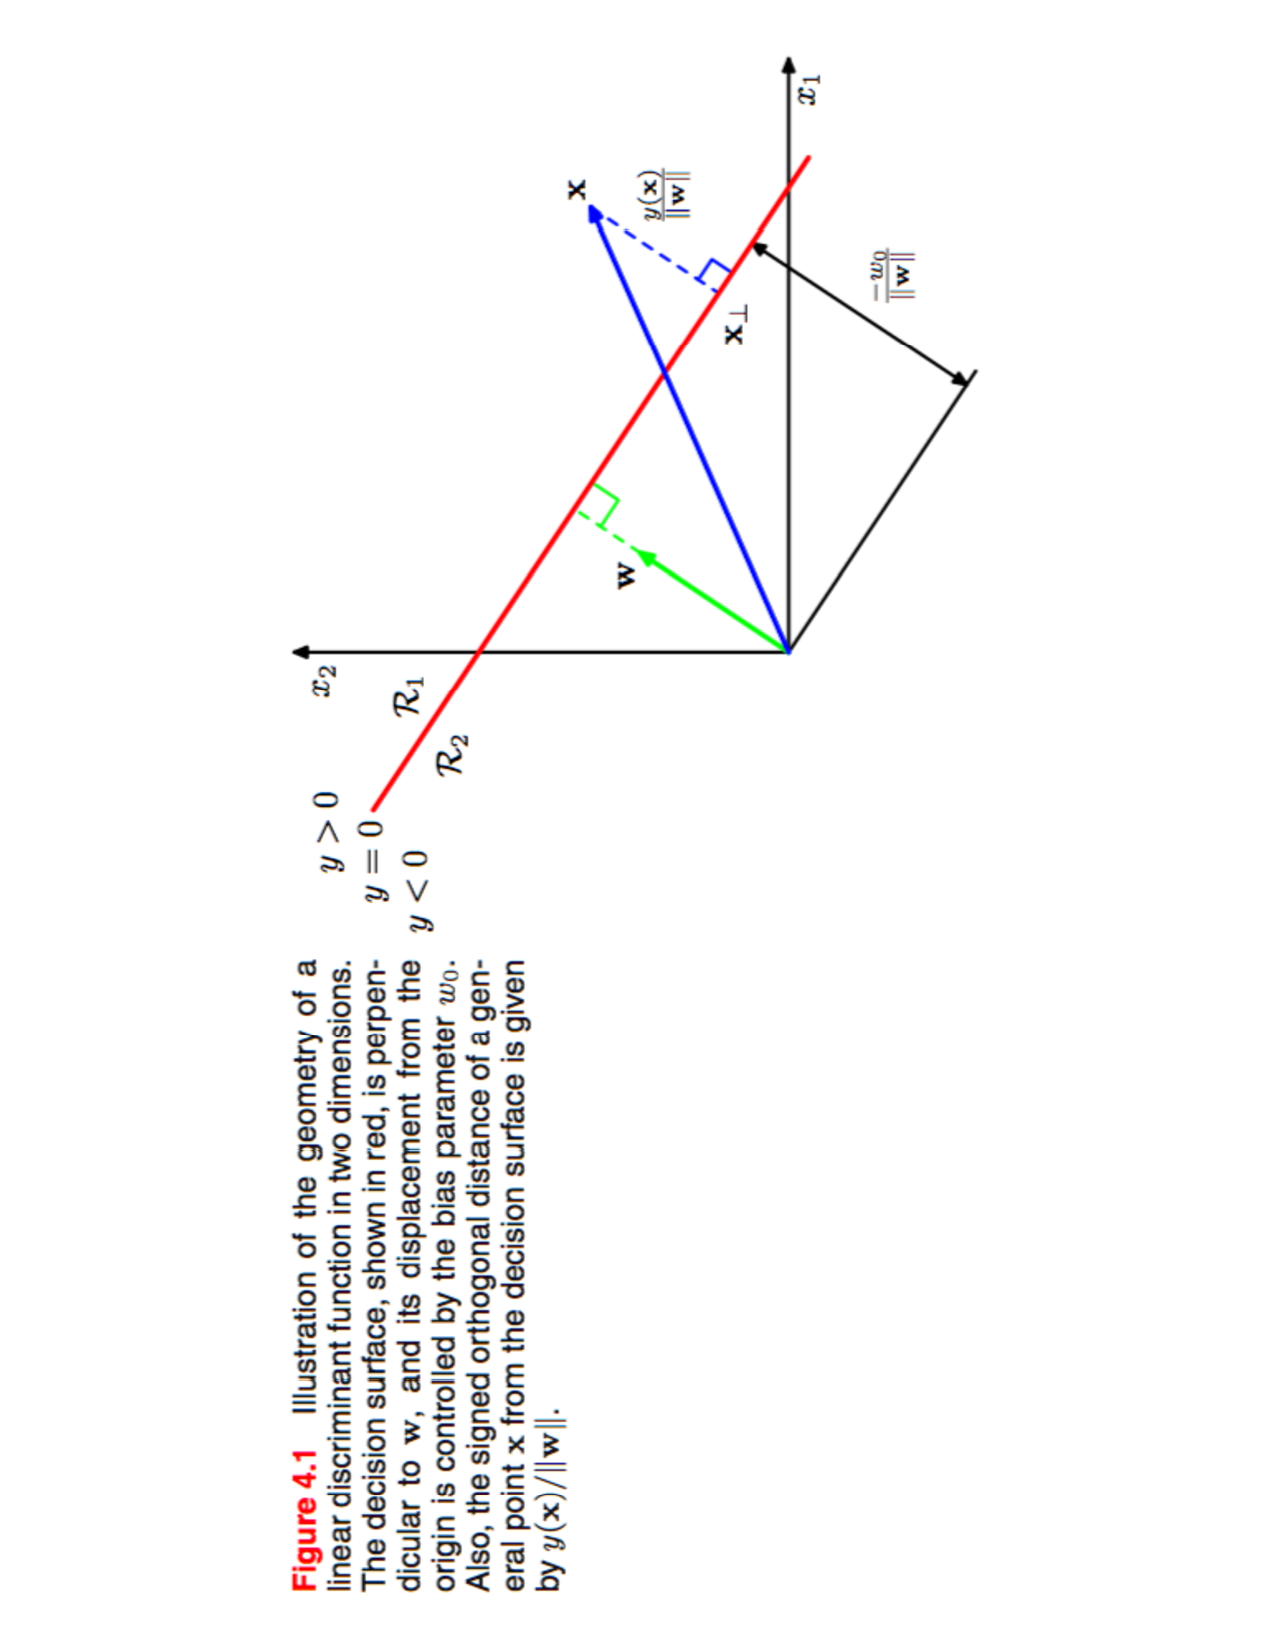
\includegraphics[width=5in, angle=270]{fig41.pdf}\end{center}

\item Let $\z$ be $\phi(\x)$
\begin{eqnarray}
y(\z) &=& \w^T\z + b \\
y(\z) &=& \w^T\left(\z_p + r \frac{\w}{\left\|w\right\|} \right) + b \\
y(\z) &=& \left(\w^T\z_p + b\right) + r \frac{\w^T\w}{\left\|w\right\|}  \\
y(\z) &=& 0 + r \frac{\w^T\w}{\left\|w\right\|}  = r \frac{\left\|w\right\|^2}{\left\|w\right\|} \\
y(\z) &=& r \left\|w\right\|  \\
\frac{y(\z)}{\left\|w\right\| } &=& r
\end{eqnarray}
\item So, the distance $r$ is $\frac{y(\z)}{\left\|w\right\| }$
\item We want $t_ny(\x_n) > 0 \forall n$:
\begin{equation}
\frac{t_ny(\x_n)}{\left\|w\right\|} = \frac{t_n\left(\w^T\phi(\x_n) + b\right)}{\left\|w\right\|} > 0
\end{equation}
\item So, we can define the following objective function:


\item Note: the figures below are from Bishop's text. 

\begin{center}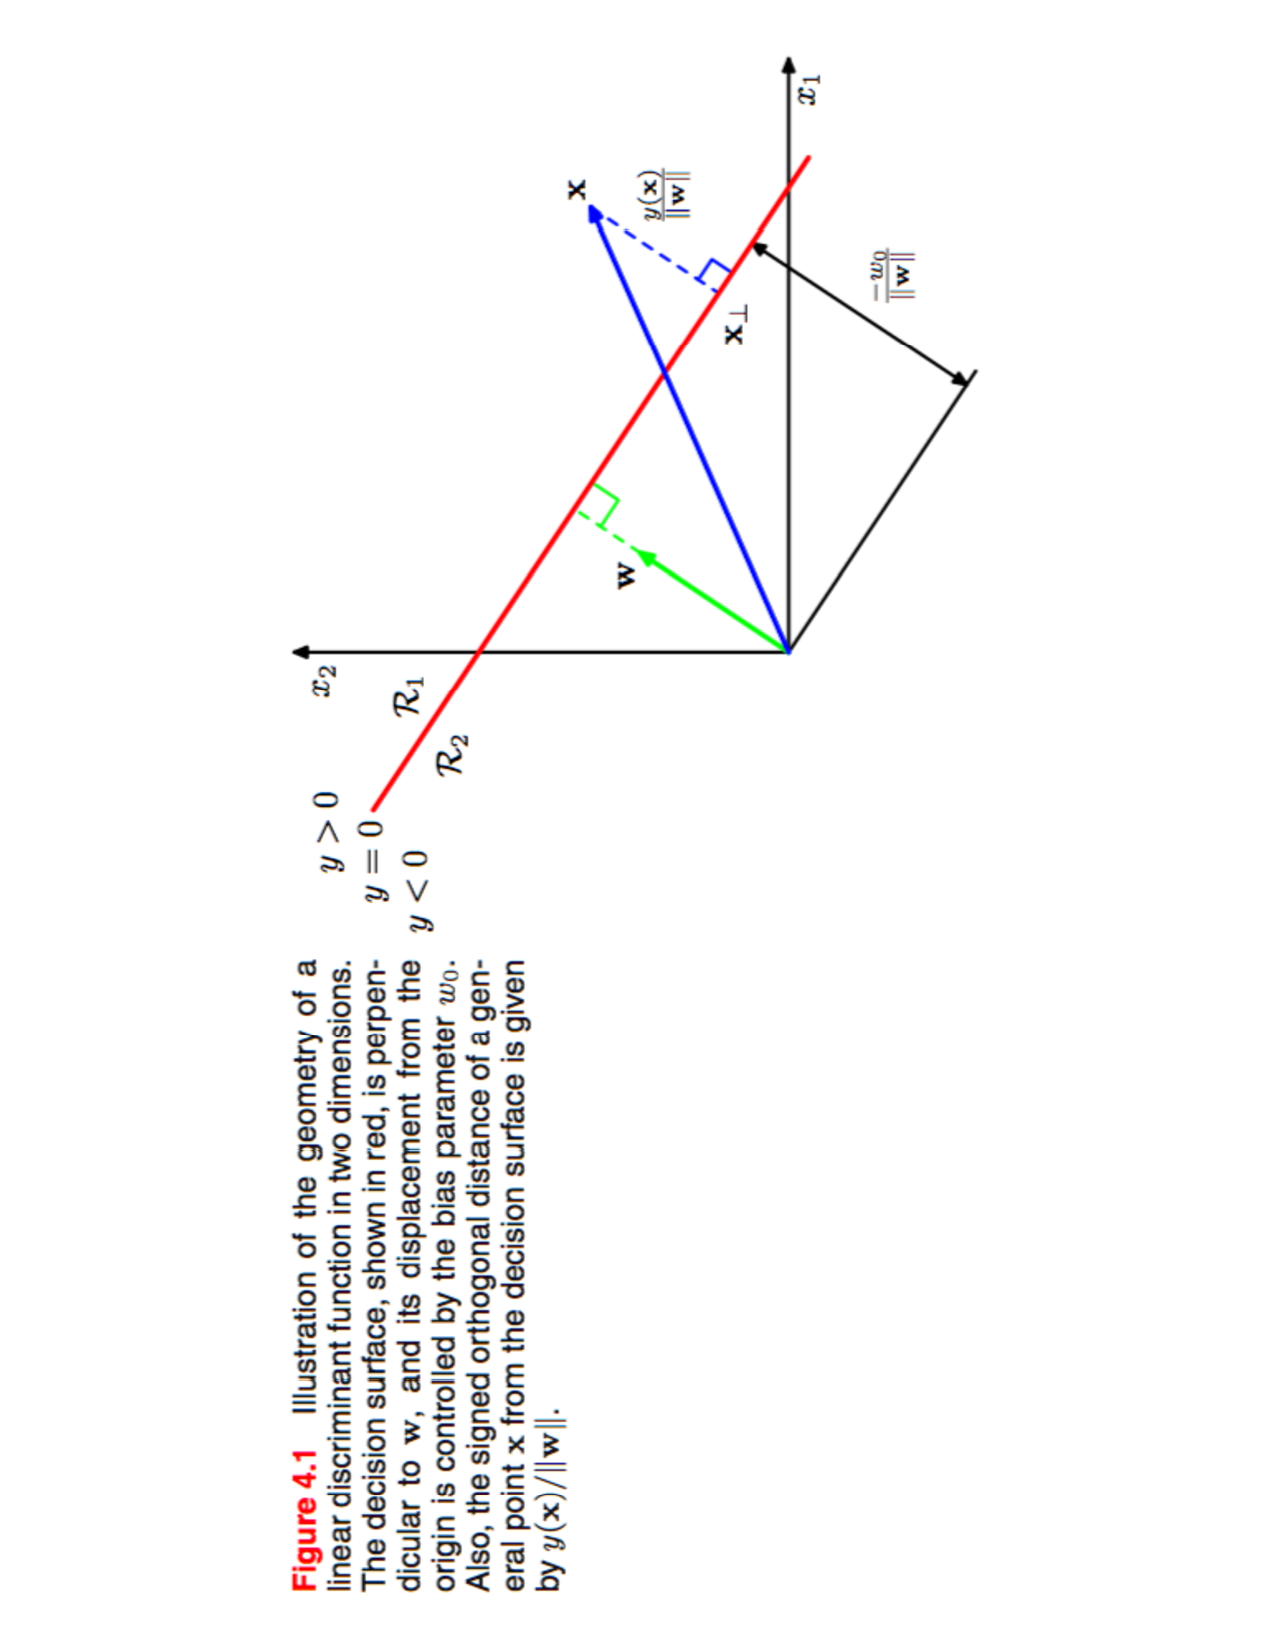
\includegraphics[width=5in, angle=270]{fig41.pdf}\end{center}

\item So, we can define the following objective function:
\begin{equation}
\arg \max_{w,b} \left\{ \frac{1}{\left\|w\right\|} \min_n \left[t_n \left(\w^T\phi(\x_n) + b \right) \right]\right\}
\end{equation}
\item We can rewrite this as a constraint.  Find the $\w$ such that $t_n\left(\w^T\phi(\x_n) + b\right) \ge 1$ for $n = 1, \ldots, N$ where $t_n\left(\w^T\phi(\x_n) + b\right) = 1$ for the smallest distances
\item Terminology: At equality, a constraint is ``active.'' At $>1$, the constraint is ``inactive''
\item Then, we can say:
\begin{equation}
\arg \min_{w,b} \frac{1}{2}\left\|\w\right\|^2 \text{ such that }  t_n \left(\w^T\phi(\x_n) + b \right)  \ge 1 \forall n
\end{equation}
\item \emph{How do we solve this?}  We use \underline{Lagrangian Optimization}
\begin{equation}
\mathscr{L}(\w,b,\mathbf{a}) =  \frac{1}{2}\left\|\w\right\|^2 - \sum_{n=1}^N a_n \left\{  t_n \left(\w^T\phi(\x_n) + b \right)  - 1 \right\}
\end{equation}
where $\mathbf{a} = \left[ a_1, \ldots, a_N\right]^T$ with $a_n \ge 0$
\item The KKT (Karush-Kuhn-Tucker conditions):
\begin{eqnarray}
t_n(\w^T\phi(\x_n) + b) -1 \ge 0\\
a_n \ge 0\\
a_n (t_n(\w^T\phi(\x_n) + b) -1 ) = 0
\end{eqnarray}


\begin{center}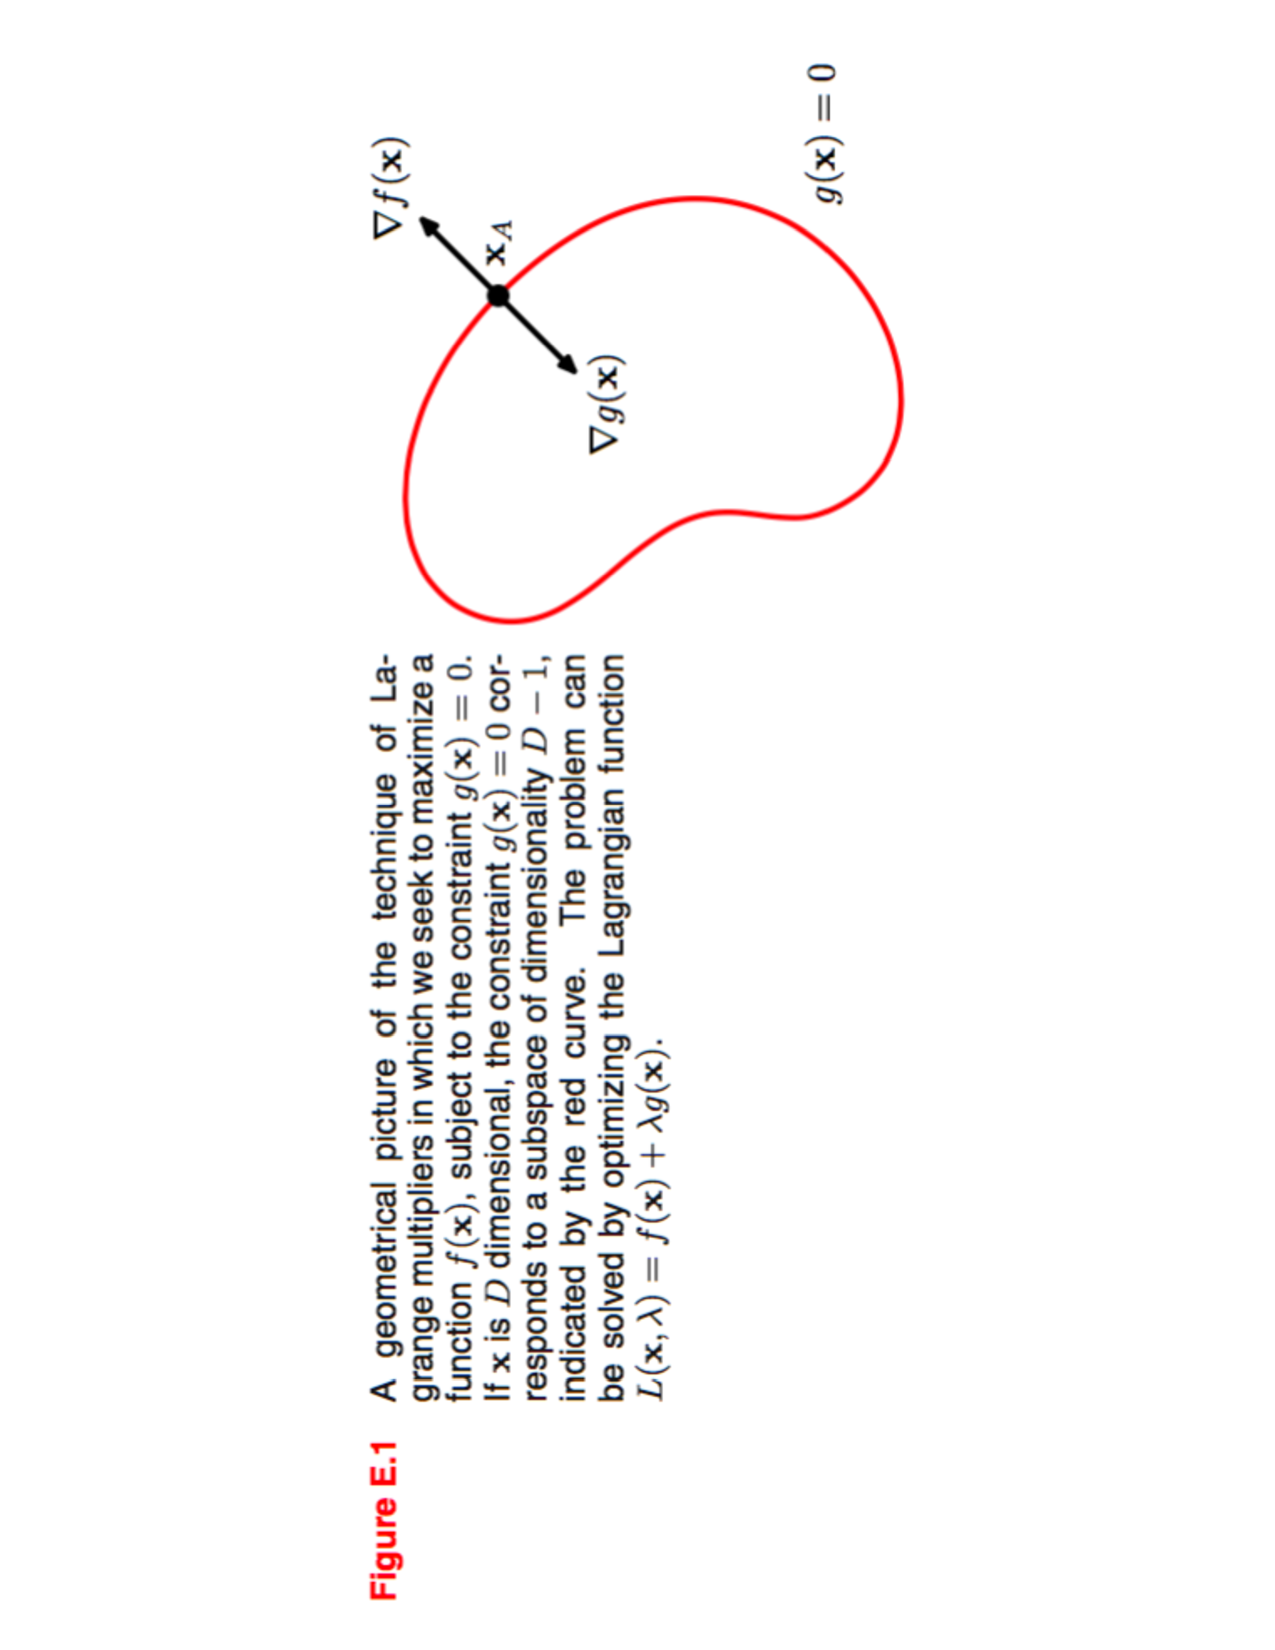
\includegraphics[width=2in, trim=5cm .5cm 4cm 1cm, clip=true, angle=270]{fig1.pdf}\end{center}


\begin{center}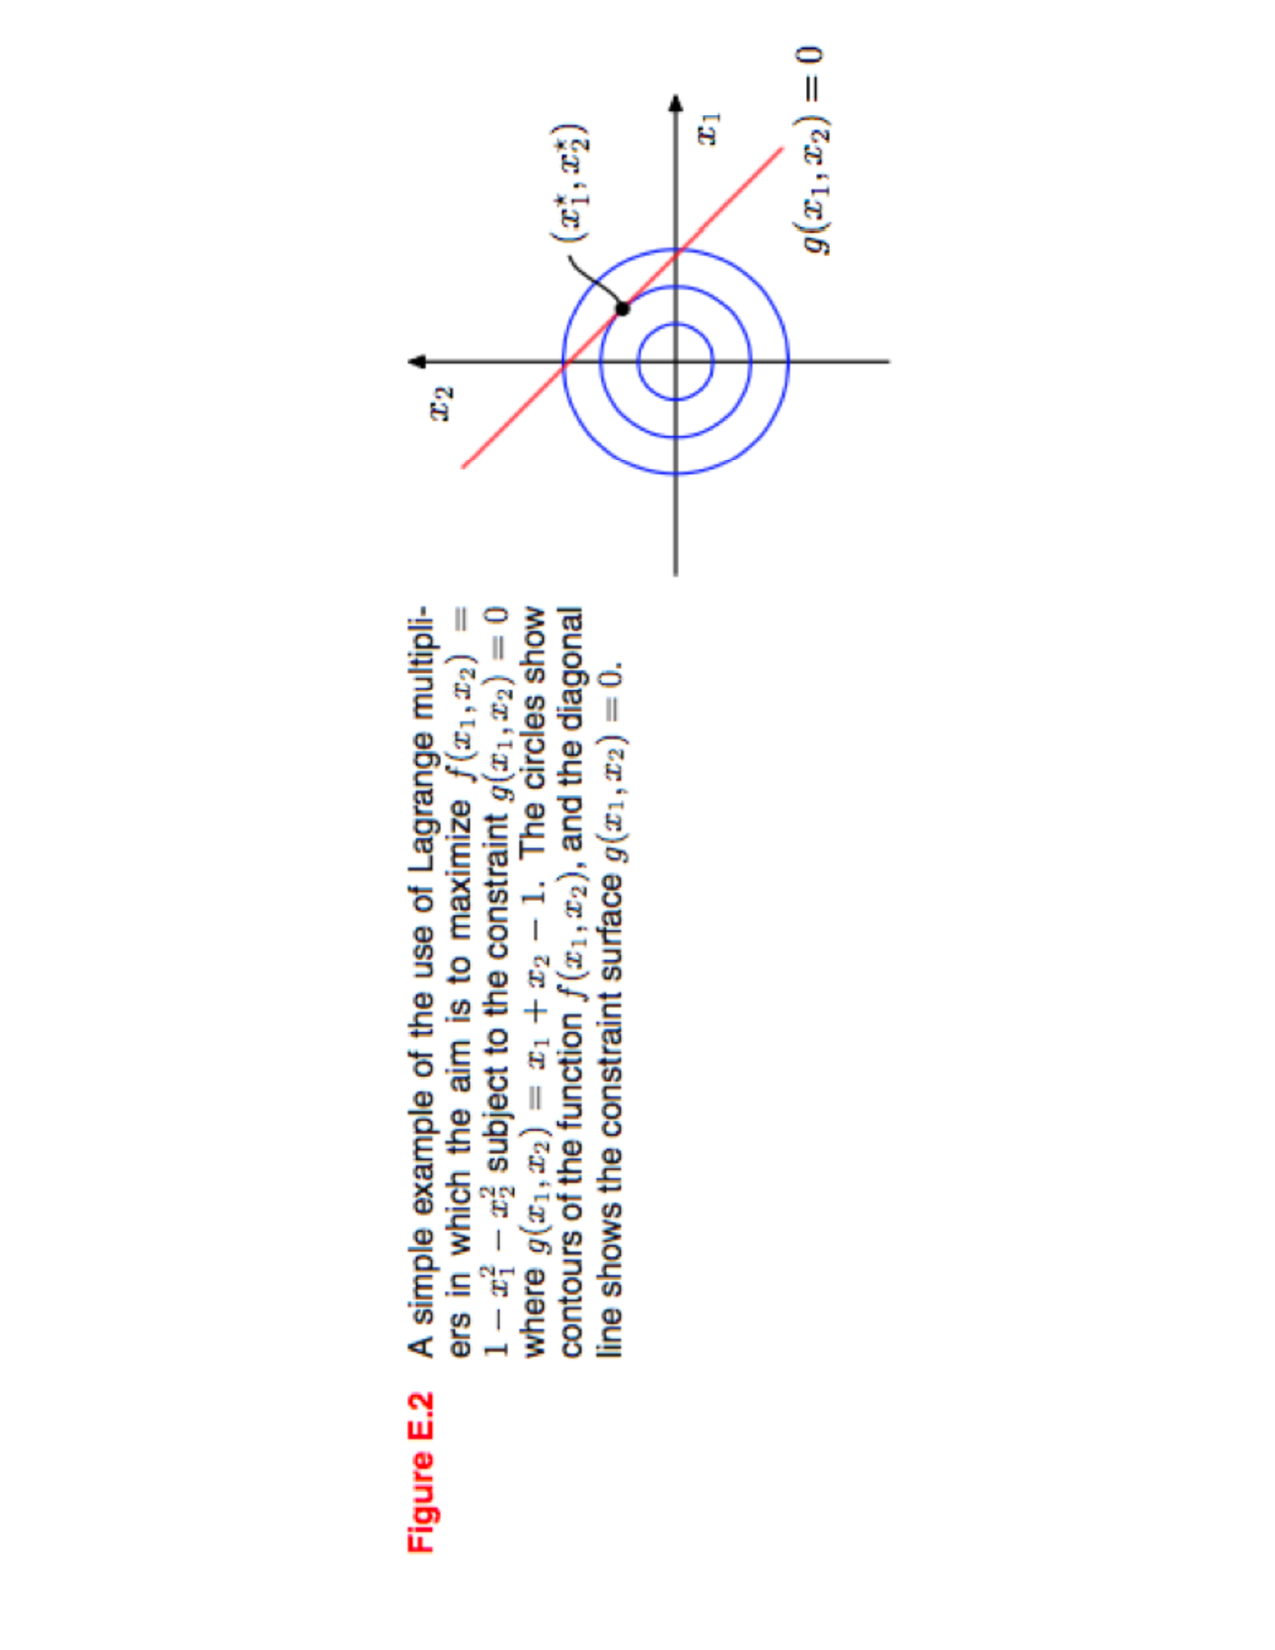
\includegraphics[width=2in, trim=5cm .5cm 4cm 2cm, clip=true, angle=270]{fig2.pdf}\end{center}

\begin{center}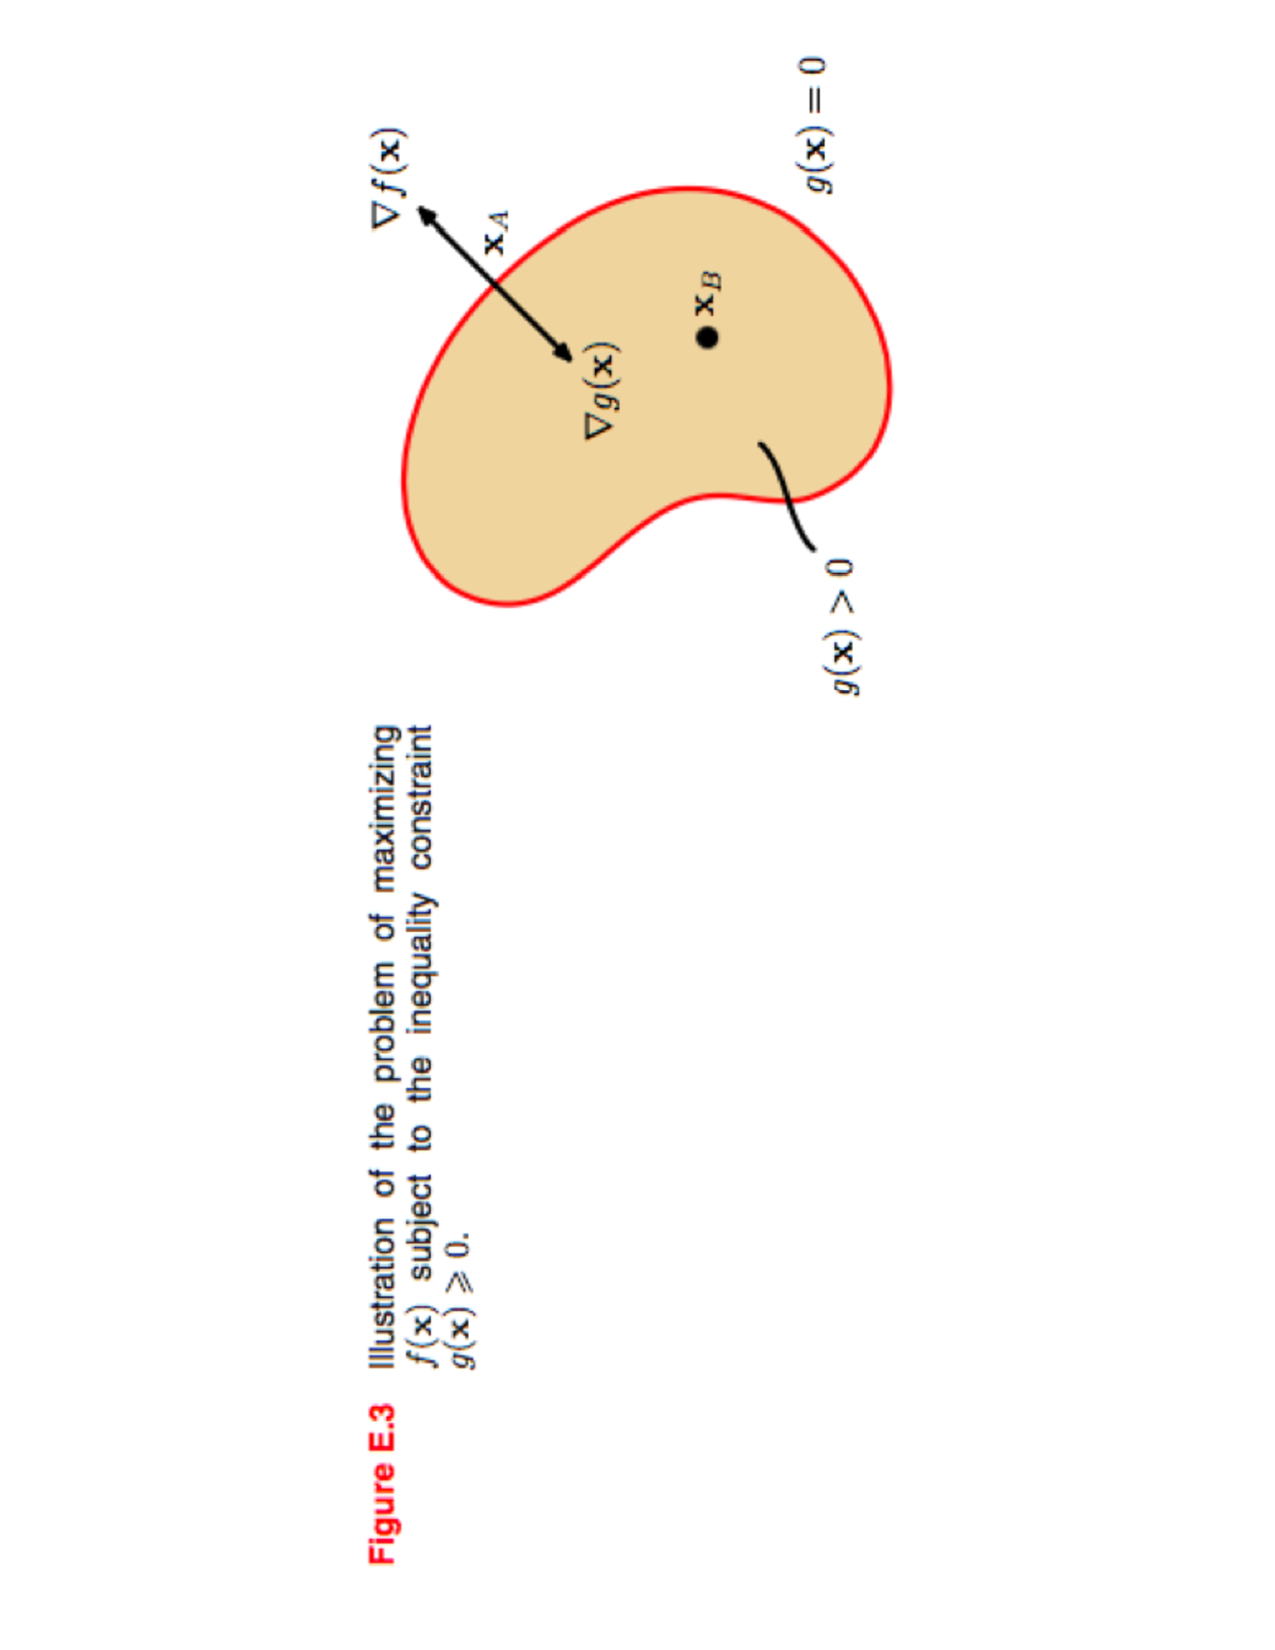
\includegraphics[width=2in, trim=5cm .5cm 4cm 1cm, clip=true, angle=270]{fig3.pdf}\end{center}


\item So, we can optimize with respect to $\w$ and $b$:
\begin{eqnarray}
\frac{\partial \mathscr{L}(\w,b,\mathbf{a})}{\w} &=& \w - \sum_{n=1}^N a_n t_n \phi(\x_n) = 0\\
\w &=& \sum_{n=1}^N a_n t_n \phi(\x_n)\\
\frac{\partial \mathscr{L}(\w,b,\mathbf{a})}{b} &=& - \sum_{n=1}^N a_n t_n  = 0\\
 \sum_{n=1}^N a_n t_n  &=& 0
\end{eqnarray}
\item We can plug these into $\mathscr{L}$
\begin{eqnarray}
\mathscr{L}(\w, b, \mathbf{a}) &=& \frac{1}{2}\w^T\w - \sum_{n=1}^N a_n \left\{  t_n \left(\w^T\phi(\x_n) + b \right)  - 1 \right\}\\
&=& \frac{1}{2}\w^T\w - \sum_{n=1}^N a_n \left\{  t_n \w^T\phi(\x_n) + t_n b   - 1 \right\}\\
&=& \frac{1}{2}\w^T\w - \sum_{n=1}^N a_n t_n \w^T\phi(\x_n) - \sum_{n=1}^N a_n t_n b   + \sum_{n=1}^N a_n \\
&=& \frac{1}{2}\w^T\w - \sum_{n=1}^N a_n t_n \w^T\phi(\x_n) - b \sum_{n=1}^N a_n t_n    + \sum_{n=1}^N a_n \\
&=& \frac{1}{2}\w^T\w - \sum_{n=1}^N a_n t_n \w^T\phi(\x_n) - 0    + \sum_{n=1}^N a_n \\
&=& \frac{1}{2}\w^T\w - \sum_{n=1}^N a_n t_n \w^T\phi(\x_n) + \sum_{n=1}^N a_n \\
\end{eqnarray}
\item Plug in for $\w$:
\begin{eqnarray}
\mathscr{L}(\w, b, \mathbf{a}) &=&  \frac{1}{2}\left(\sum_{n=1}^N a_n t_n \phi(\x_n) \right)^T\left(\sum_{n=1}^N a_n t_n \phi(\x_n) \right)- \sum_{n=1}^N a_n t_n \left(\sum_{n=1}^N a_n t_n \phi(\x_n) \right)^T\phi(\x_n) + \sum_{n=1}^N a_n \nonumber \\
&=& \frac{1}{2} \sum_{i=1}^N\sum_{j=1}^N a_i a_j t_i t_j \phi(\x_i)^T\phi(\x_j) - \sum_{i=1}^N\sum_{j=1}^N a_i a_j t_i t_j \phi(\x_i)^T\phi(\x_j) + \sum_{n=1}^N a_n \nonumber \\
&=& \sum_{n=1}^N a_n - \frac{1}{2} \sum_{i=1}^N\sum_{j=1}^N a_i a_j t_i t_j \phi(\x_i)^T\phi(\x_j) \nonumber\\
&=& \sum_{n=1}^N a_n - \frac{1}{2} \sum_{i=1}^N\sum_{j=1}^N a_i a_j t_i t_j \K(\x_i,\x_j) \nonumber
\end{eqnarray}
\item This gives us the dual.  We want to maximize this wrt $a_i$:
\begin{equation}
\max_{\mathbf{a}} \mathscr{L}(\mathbf{a}) = \sum_{n=1}^N a_n - \frac{1}{2} \sum_{i=1}^N\sum_{j=1}^N a_i a_j t_i t_j \K(\x_i,\x_j) \text{ such that } a_n \ge 0, \sum_{n=1}^N a_nt_n = 0
\end{equation}
\item This is a quadratic programming problem:  A quadratic objective with linear constraints
\item We can plug into y with out solved $\w$ form: $y(\x) = \sum_{n=1}^N a_nt_n\K(\x,\x_n) + b$
\item We can look at the KKT conditions for the dual:
\begin{eqnarray}
t_ny(\x_n) -1 \ge 0\\
a_n \ge 0\\
a_n (t_ny(\x_n) -1 ) = 0
\end{eqnarray}
\item Either $a_n =0$ or $t_ny(\x_n) = 1$.  When $t_ny(\x_n) = 1$, then $\x_n$ is a support vector. 
\item Using $t_ny(\x_n) =1$ for support vectors, we can solve for $b$.
\begin{equation}
t_n\left( \sum_{m \in S} a_mt_m\K(\x_n, \x_m) \right) = 1
\end{equation}
\item Average over all S.V.s: 
\begin{equation}
b = \frac{1}{N_S} \sum_{n\in S} \left( t_n - \sum_{m \in S} a_mt_m\K(\x_n, \x_m) \right) 
\end{equation}
 because:
\begin{eqnarray}
& & t_n\left[t_n\left( \sum_{m \in S} a_mt_m\K(\x_n, \x_m) + b\right)\right] = (1)t_n\\
& &  \sum_{m \in S} a_mt_m\K(\x_n, \x_m) + b = t_n\\
& & b = t_n -  \sum_{m \in S} a_mt_m\K(\x_n, \x_m)
\end{eqnarray}
\end{itemize}


\end{document} 